\documentclass[]{article}
% bib use
\usepackage{cite}
% tabular eqn
\usepackage{amsmath, array}
% code listing
\usepackage{listings}
% images
\usepackage{graphicx} 
% lock images
\usepackage{float}
% colored syntax highlighting
\usepackage{xcolor}  
%captions in listings
\usepackage{caption}
% multirows in tables
\usepackage{multirow}
%longtable
\usepackage{array}
\usepackage{longtable}
%mathbb
\usepackage{amsfonts}


%opening
\title{Principles of statistical inference project - Part 2}
\author{Carmel Gafaż}

\begin{document}

\maketitle

% style for all code snippets
\lstset{
	basicstyle=\ttfamily\footnotesize,  % Use Courier (monospace)
	numbers=left, numberstyle=\tiny, stepnumber=1, numbersep=5pt,
	breaklines=true, breakatwhitespace=true,
	frame=single, rulecolor=\color{gray}  % Single-line frame
}


\section{Question 1}

\textbf{Find and download a dataset from the internet that includes at least three quantitative
variables (more is better). Once you have selected a dataset, send the link via email to Dr.
Monique Borg Inguanez (monique.inguanez@um.edu.mt) for approval, ensuring that each
student works with a unique dataset.
Using the approved dataset, fit a Bayesian multiple linear regression model (p < 2) using
JAGS.
Your submission should clearly include the following:}

\bigskip

The selected dataset is the Concrete Compressive Strength dataset, which was downloaded from the University of California, Irvine. The response variable of the dataset is the Concrete compressive strength as a function of eight predictors, including ingredients and ageing time.

The following table outlines the variables of the dataset, which had no missing values:

\begin{table}[H]
	\centering
	\begin{tabular}{|l|l|l|l|}
		\hline
		\textbf{Variable Name} & \textbf{Role} & \textbf{Type} & \textbf{Units} \\ \hline
		Cement                 & Feature       & Continuous     & kg/m\textsuperscript{3} \\ \hline
		Blast Furnace Slag     & Feature       & Integer        & kg/m\textsuperscript{3} \\ \hline
		Fly \texttt{ash}                & Feature       & Continuous     & kg/m\textsuperscript{3} \\ \hline
		Water                  & Feature       & Continuous     & kg/m\textsuperscript{3} \\ \hline
		Superplasticizer       & Feature       & Continuous     & kg/m\textsuperscript{3} \\ \hline
		Coarse Aggregate       & Feature       & Continuous     & kg/m\textsuperscript{3} \\ \hline
		Fine Aggregate         & Feature       & Continuous     & kg/m\textsuperscript{3} \\ \hline
		Age                    & Feature       & Integer        & day \\ \hline
		Concrete Compressive Strength & Target & Continuous     & MPa \\ \hline
	\end{tabular}
	\caption{Variables in the Concrete Compressive Strength dataset}
	\label{tab:concrete_variables}
\end{table}

A first test on the dataset involved a pairwise and visual inspection of the relationships to determine the correlation of the predictors with the response and to start forming some ideas about multicollinearity. These results are shown below in Figure \ref{fig:img-pairwise-numeric} and Figure \ref{fig:img-pairwise-plot}.



\begin{figure}[H]
	\centering
	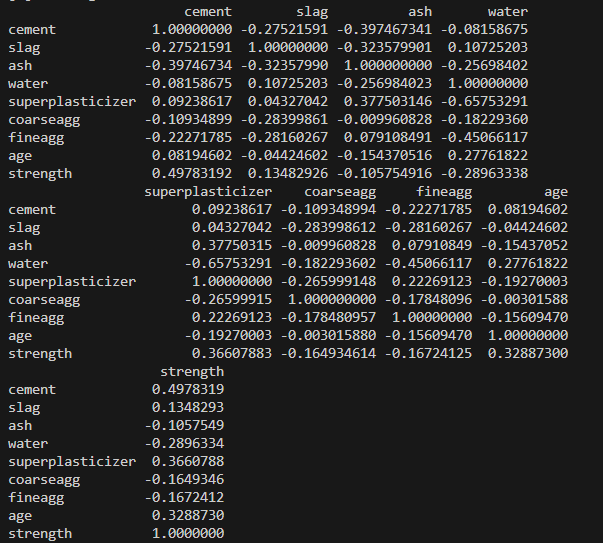
\includegraphics[width=0.5\linewidth]{img/img-pairwise-numeric}
	\caption{ Correlation matrix of all variables in the Concrete Compressive Strength dataset. }
	\label{fig:img-pairwise-numeric}
\end{figure}


\begin{figure}[H]
	\centering
	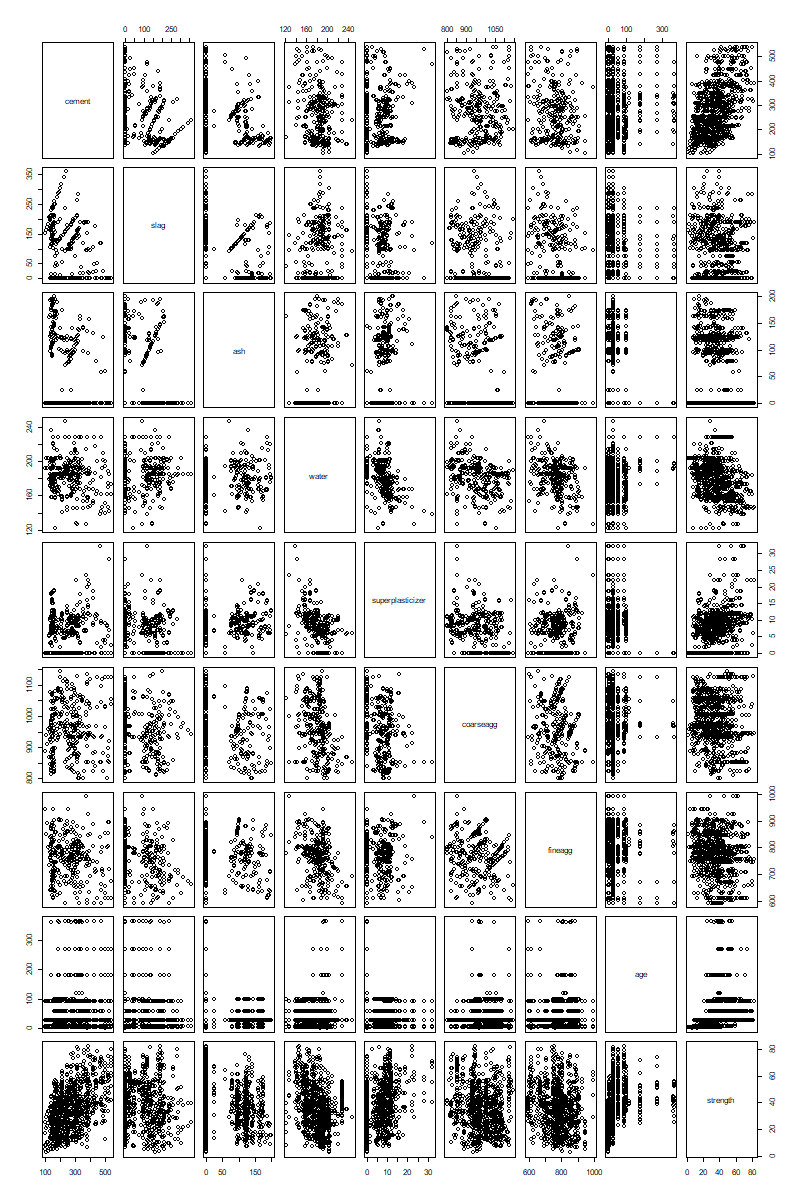
\includegraphics[width=0.5\linewidth]{img/img-pairwise-plot}
	\caption{Pairwise scatterplot matrix of all variables in the Concrete Compressive Strength dataset.}
	\label{fig:img-pairwise-plot}
\end{figure}


From this result, the best correlation with strength is achieved with \texttt{cement}, followed by a moderate correlation with \texttt{superplasticiser} (+0.37) and \texttt{age} (+0.33).
Water has a moderate negative correlation (-0.29). \texttt{Slag} and \texttt{ash} have a weak correlation. We can also see a strong negative correlation between \texttt{superplasticiser} and \texttt{water} (-0.66) and \texttt{water} and \texttt{fine aggregate} (-0.45).


Variance inflation factor analysis was then conducted to investigate multicollinearity, with the results of the analysis presented in Figure \ref{fig:img-vif}.

\begin{figure}
	\centering
	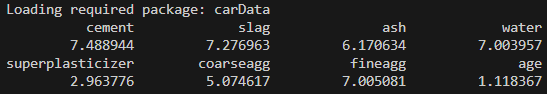
\includegraphics[width=0.7\linewidth]{img/img-vif}
	\caption{Variance Inflation Factor values for all predictors in the Concrete Compressive Strength dataset.}
	\label{fig:img-vif}
\end{figure}



The analysis shows that cement,  \texttt{Slag}, \texttt{ash}, and \texttt{water} exhibit high collinearity (in the region of 7), while \texttt{superplasticiser} (2.96) and  \texttt{age} (1.12) have moderate values.

Following this investigation, cement, \texttt{superplasticiser}, and \texttt{age} were selected as predictors.


The following code snippet illustrates the data preparation. Prior to this step, the datasets's column names were shortened so they could be manipulated easily.

\begin{lstlisting}
script_dir <- getwd()
concrete_cleansed_path <- file.path(
script_dir, "project_2_code/concrete_cleansed.csv")

concrete_cleansed <- read.csv(concrete_cleansed_path)

jags_data <- list(
x_cement = concrete_cleansed$cement,
x_superplasticizer = concrete_cleansed$superplasticizer,
x_age = concrete_cleansed$age,
y_strength = concrete_cleansed$strength,
n = nrow(concrete_cleansed)
)
\end{lstlisting}




\subsection{A full specification of the Bayesian model:}
\textbf{\begin{itemize}
	\item The likelihood function
	\item The prior distributions selected for the parameters
\end{itemize}}



The response variable in this excercise is \texttt{strength}, representing the concrete compressive strength in MPa. As we have seen in the previous section, the predictors included in the model are \texttt{cement}, \texttt{superplasticizer}, and \texttt{age}, all selected based on correlation and multicollinearity analysis.

The model assumes the following structure:

\begin{flalign*}
	y_i &\sim \mathcal{N}(\mu_i, \tau^{-1}) \quad \text{for } i = 1, \dots, n \\
	\mu_i &= \beta_0 + \beta_1 \cdot x_{\text{cement}, i} + \beta_2 \cdot x_{\text{superplasticizer}, i} + \beta_3 \cdot x_{\text{age}, i}
\end{flalign*}

The prior distributions for the parameters are defined as follows:

\begin{align*}
	\beta_0 &\sim \mathcal{N}(0, 100) \\
	\beta_1 &\sim \mathcal{N}(0, 100) \\
	\beta_2 &\sim \mathcal{N}(0, 100) \\
	\beta_3 &\sim \mathcal{N}(0, 100) \\
	\tau &\sim \text{Gamma}(0.01, 0.01)
\end{align*}

The variance of the likelihood is modeled via the precision parameter $\tau$, where;
$$
\tau = \frac{1}{\sigma^2}
$$

The model was defined using the following statement:

\begin{lstlisting}
model_description <- "
model {
	for (i in 1:n) {
		y_strength[i] ~ dnorm(mu[i], tau)
		mu[i] <- beta0 + (beta1 * x_cement[i]) + (beta2 * x_superplasticizer[i]) + (beta3 * x_age[i])
	}
	beta0 ~ dnorm(0, 0.01)
	beta1 ~ dnorm(0, 0.01)
	beta2 ~ dnorm(0, 0.01)
	beta3 ~ dnorm(0, 0.01)
	tau ~ dgamma(0.01, 0.01)
} "
		
\end{lstlisting}



\subsection{A justification for the chosen priors, including any assumptions or reasoning behind
them.}


The priors in this model are weakly informative; that is, they do not strongly influence the results, but they give only a little information about what values we expect for the parameters. The coefficients for $\beta$, for example, were given normal priors centred at 0 with a standard deviation of 10, which allows for a large range of possible values. These priors are wide enough to let the data have the biggest impact on the results, but they also help the model stay stable and avoid extreme or unrealistic values during sampling.

\begin{itemize}
	\item \textbf{Regression Coefficients ($\beta_0$, $\beta_1$, $\beta_2$, $\beta_3$):} Each coefficient was assigned a normal prior $\mathcal{N}(0, 100)$, corresponding to a mean of 0 and a large variance of 100, reflecting a belief that the effect of each predictor is centred around zero but allows for a wide range of plausible values. As discussed, these priors are considered weakly informative because they do not strongly constrain the parameter estimates but prevent extreme values that could destabilize the sampling process.
	
	\item \textbf{Precision Parameter ($\tau$):} A Gamma$(0.01, 0.01)$ prior was used for the precision of the normal likelihood, which is a standard weak prior for precision in Bayesian models. It gives a very wide range of possible values for the standard deviation, which means we do not assume much about how spread out the data is, reflecting that we have little prior knowledge about the variation in the response.
\end{itemize}

The priors were selected to reflect minimal assumptions about the parameter values in the absence of strong domain knowledge, which is appropriate given the exploratory nature of this analysis.

\subsection{The selected burn-in period for your MCMC chains, including a detailed explanation
of how this was chosen.}

In Bayesian analysis using Markov Chain Monte Carlo, the initial samples of each chain will, in most cases, not reflect the target posterior distribution, and the chain will settle into the posterior distribution after a number of samples. This early phase is known as the burn-in period. These initial samples are discarded before subsequent analysis, as they would bias the results.

Trace plots are the first tool that is used to determine a suitable burn-in period. In this analysis, we examine chain mixing, which the overlap of the chain samples can visually assess, and compactness within the chain samples. Additionally, chain variations should be consistent around a central value. Trace plots, however, are subjective in interpretation and can indicate early convergence. Another tool that is then used is the Gelman-Rubin convergence diagnostic, which utilises both between-chain and within-chain variance to assess convergence.

Figure~\ref{fig:img-trace-beta0} shows the trace plot for the parameter $\beta_0$, that is, the intercept after a burn-in of just 200 samples. The trance can visually satisfy the criteria for convergence.

\begin{figure}[H]
	\centering
	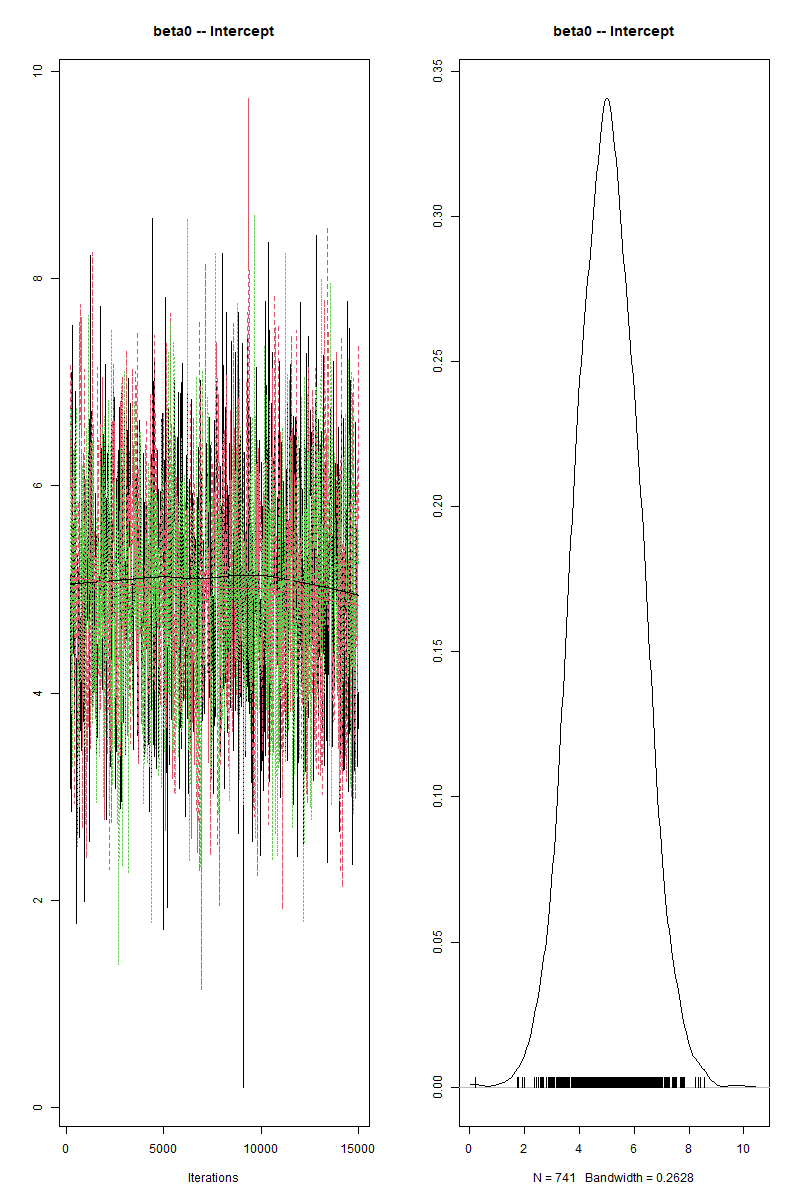
\includegraphics[width=0.7\linewidth]{img/img-trace-beta0}
	\caption{Trace and density plot for $\beta_0$ (Intercept) across 3 chains after iteration 200.}
	\label{fig:img-trace-beta0}
\end{figure}


The Gelman-Rubin diagnostic was also examined. Figure~\ref{fig:img-gelman-plot-beta0} shows that the values for all parameters converge to 1.00 after iteration 6000, confirming chain convergence and the initial iterations were likely influenced by starting values.

\begin{figure}[H]
	\centering
	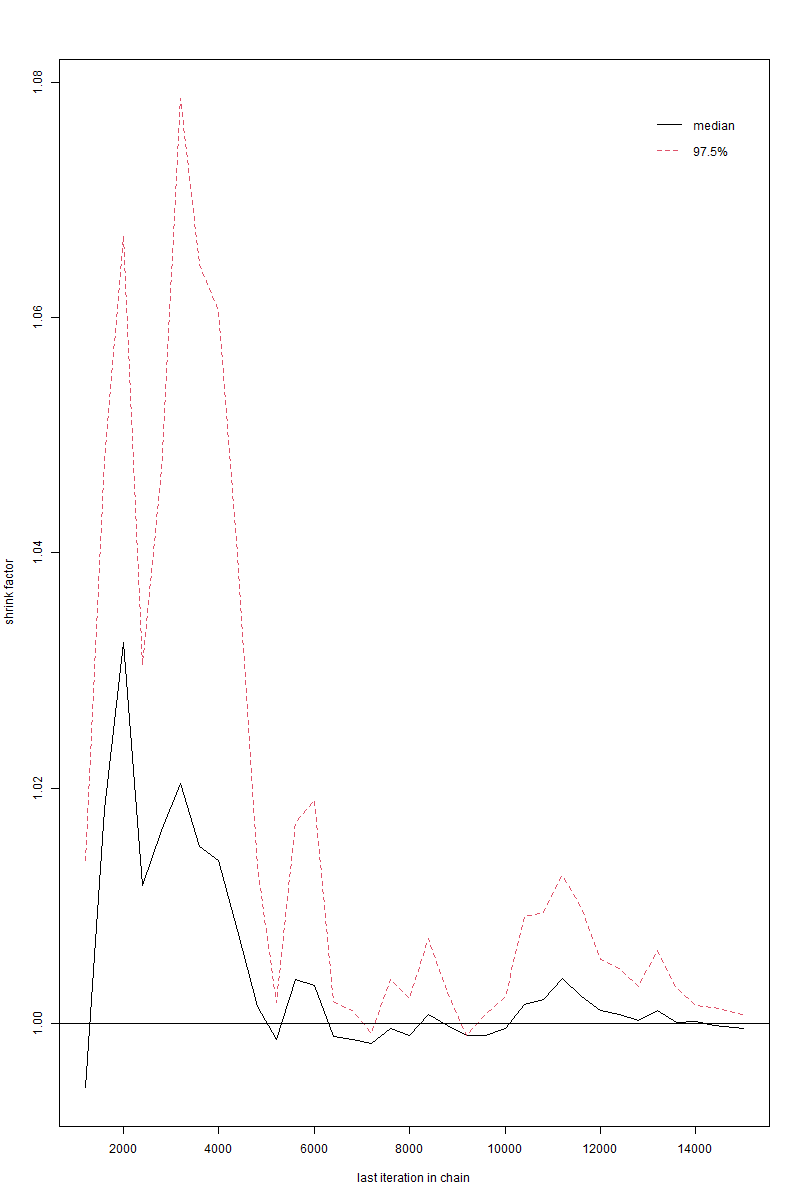
\includegraphics[width=0.7\linewidth]{img/img-gelman-plot-beta0}
	\caption{Gelman--Rubin diagnostic for $\beta_0$. Convergence is reached after approximately 6000 iterations}
	\label{fig:img-gelman-plot-beta0}
\end{figure}


Based on these observations, a burn-in of 6000 iterations was selected to ensure that only samples drawn from the stationary portion of the chains were retained for posterior inference.


The following snippet shows the execution of the model and creation of the plot used in this analysis

\begin{lstlisting}
n_chains <- 3
n_burnin <- 200
n_samples <- 15000
parameters_to_monitor <- c("beta0", "beta1", "beta2", "beta3", "tau")

initial_values <- list(
list(beta0 = -10, beta1 = 0.5, beta2 = 0.1, beta3 = 0.05, tau = 0.5),
list(beta0 = 0,   beta1 = 1,   beta2 = 0.3, beta3 = 0.1,  tau = 1),
list(beta0 = 10,  beta1 = 2,   beta2 = 0.5, beta3 = 0.2,  tau = 2)
)

model <- jags.model(textConnection(model_description),
data = jags_data,
inits = initial_values,
n.chains = n_chains)

post <- coda.samples(model = model,
variable.names = parameters_to_monitor,
n.iter = n_samples,
thin = 20)

post_burned <- window(post, start = n_burnin)
print(summary(post_burned))
plot(post_burned[, "beta0"], main="beta0 -- Intercept")
\end{lstlisting}



\subsection{A presentation and interpretation of:}
\textbf{\begin{itemize}
	\item Convergence diagnostics (e.g., trace plots, Gelman-Rubin statistics)
	\item Accuracy diagnostics (e.g., effective sample size, autocorrelation)
\end{itemize}}


The Figures below illustrate convergence diagnostics for all monitored parameters in the model. Trace plots are shown after discarding an initial burn-in of 200 samples, highlighting chain behaviour and visual mixing. Additionally, Gelman-Rubin diagnostic plots are presented both after a burn-in of 200 samples and after a more conservative burn-in of 6000 samples. These plots allow for a comparative evaluation of convergence, confirming that the longer burn-in more effectively removed transient behaviour and yielded PSRF values stabilising around 1.00 across all parameters.


\begin{figure}[H]
	\centering
	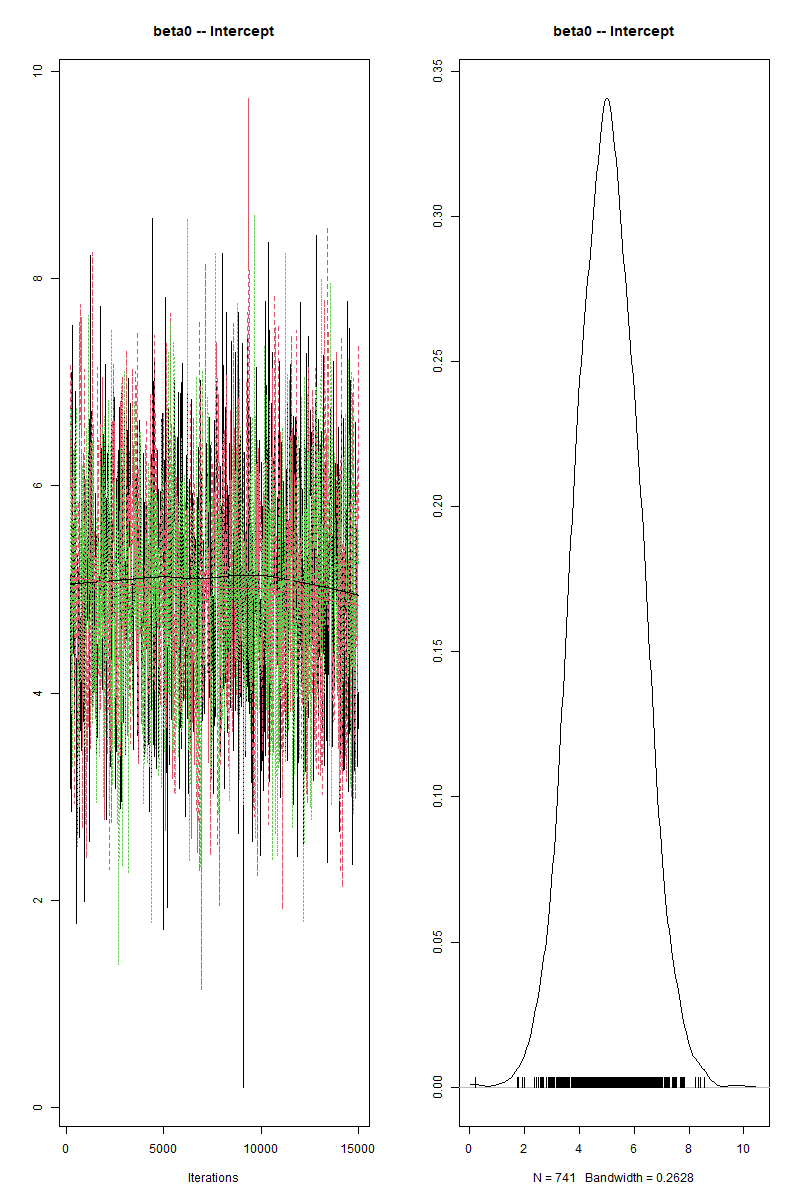
\includegraphics[width=0.7\linewidth]{img/img-trace-beta0}
	\caption{Trace and posterior density plots for the parameter $\beta_0$ (Intercept). The trace plot shows samples from three chains with good mixing and no signs of divergence or drift. All chains fluctuate around a common central value and remain tightly overlapped throughout the sampling period, a sign of stable convergence. The density plot shows a unimodal posterior distribution, peaking near 5.0 and spanning a broad range from approximately 2 to 8. The shape of the curve is slightly asymmetric near the peak, but remains smooth overall. The rug plot confirms dense and well-distributed sampling, supporting a reliable estimate of the intercept parameter. This indicates that the model has effectively identified a stable posterior distribution for $\beta_0$.}
	\end{figure}


\begin{figure}[H]
	\centering
	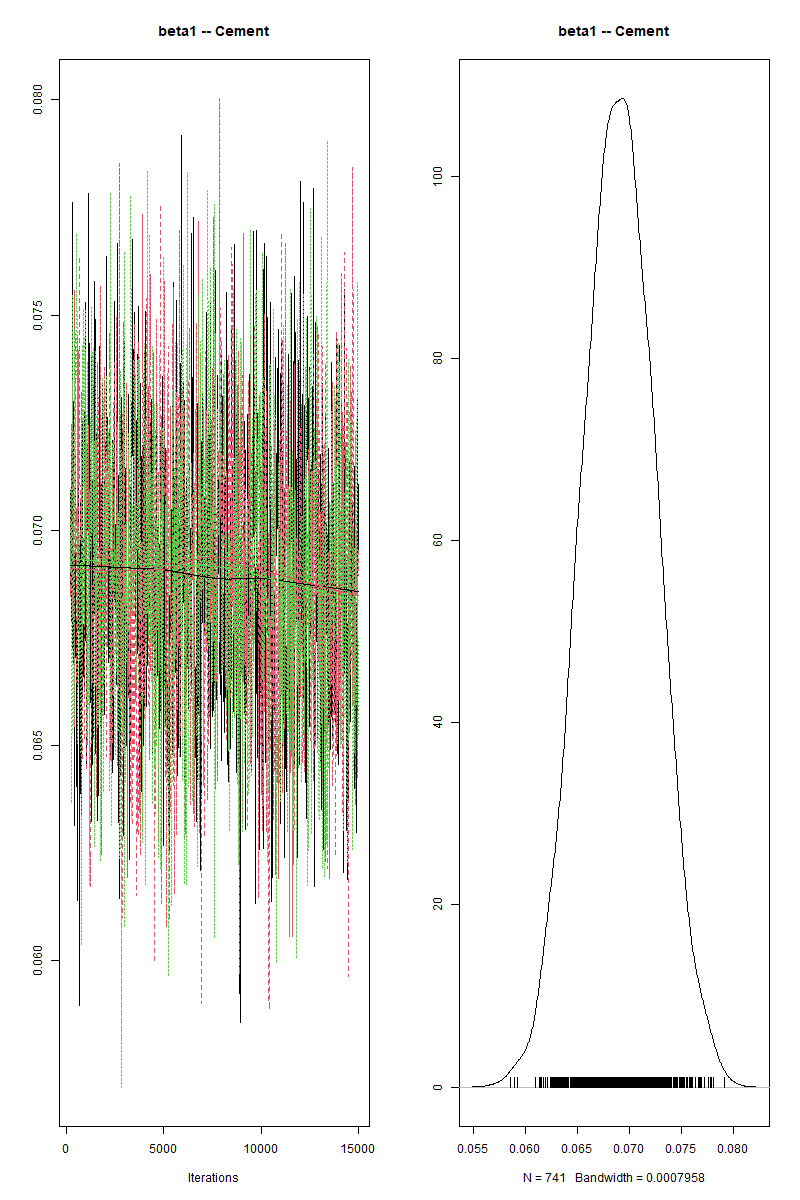
\includegraphics[width=0.7\linewidth]{img/img-trace-beta1}
	\caption{Trace and posterior density plots for the parameter $\beta_1$ (Cement). The trace plot on the left displays samples from three Markov Chain Monte Carlo (MCMC) chains. These chains show good mixing, with overlapping fluctuations around a stable mean after a burn-in period of 200 iterations. There is no visible drift or separation between the chains, and each chain explores the same region of the parameter space, indicating that convergence for $\beta_1$ has been achieved. The density plot on the right illustrates a smooth, unimodal posterior distribution, with the majority of the probability mass concentrated between approximately 0.060 and 0.078, peaking near 0.069. This suggests a strong positive effect of cement on concrete compressive strength.}
	\label{fig:img-trace-beta1}
\end{figure}

\begin{figure}[H]
	\centering
	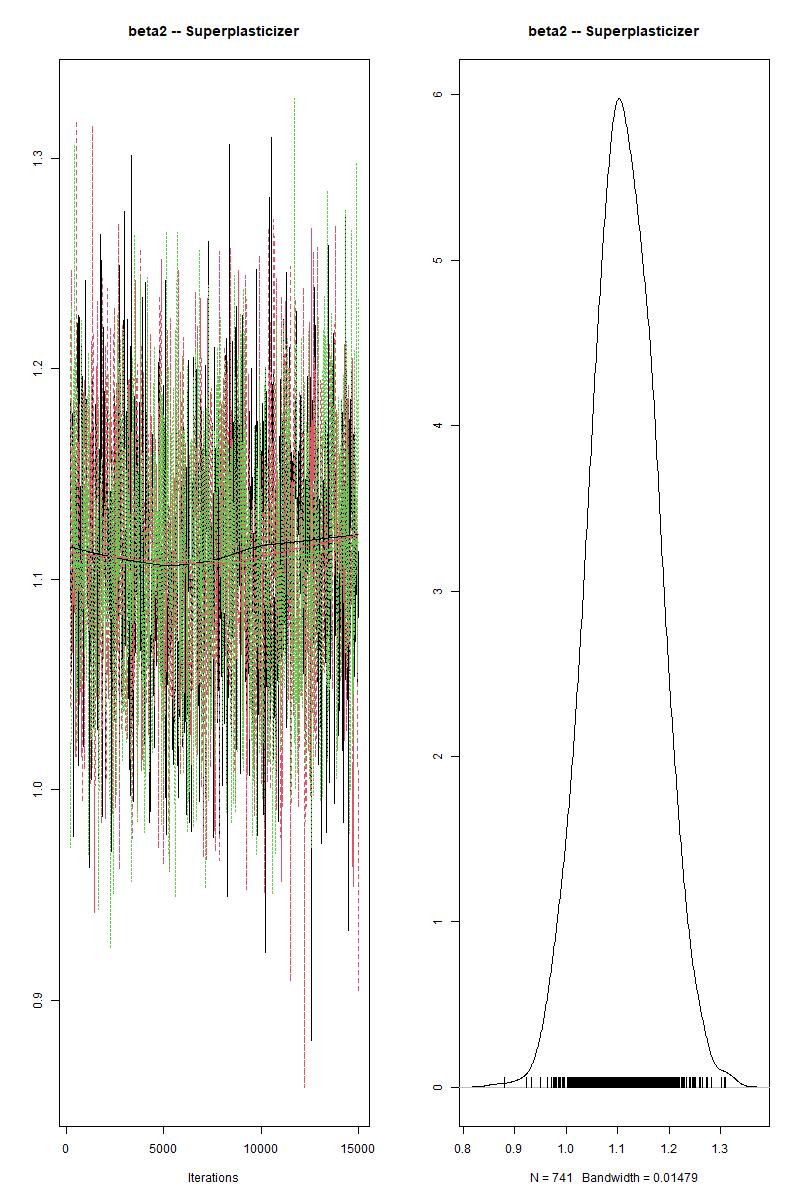
\includegraphics[width=0.7\linewidth]{img/img-trace-beta2}
	\caption{Trace and posterior density plots for the parameter $\beta_2$ (Superplasticizer). The trace plot shows three well-mixed chains with no indications of divergence, upward drift, or chain separation. The chains overlap consistently and fluctuate around a common mean, showing convergence and stationarity. The posterior density plot is unimodal, with the distribution between approximately 0.95 and 1.25, and a peak near 1.11. The curve is slightly asymmetric, with a marginally longer right tail, indicating slight skewness in the posterior. The rug plot confirms that sampling was dense and thorough across the high-probability region. These results indicate a stable and significant positive effect of superplasticizer on concrete compressive strength.}
	\label{fig:img-trace-beta2}
\end{figure}

\begin{figure}[H]
	\centering
	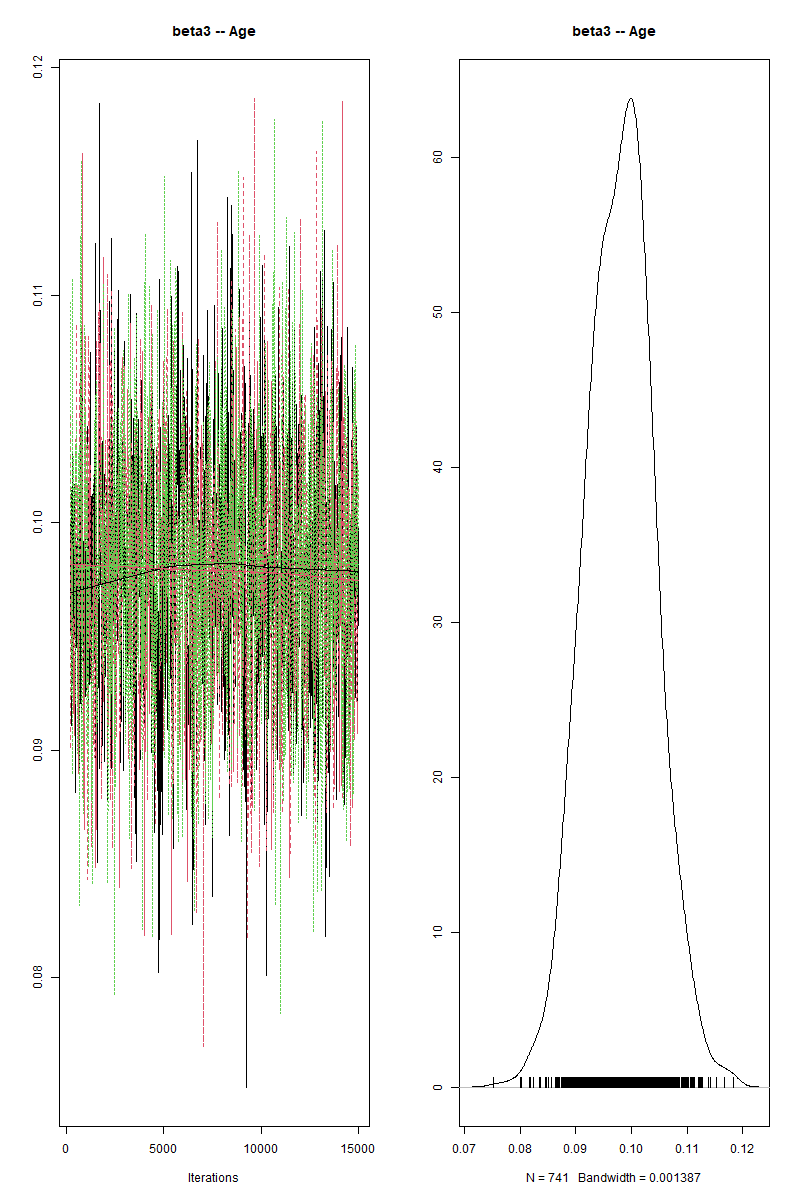
\includegraphics[width=0.7\linewidth]{img/img-trace-beta3}
	\caption{Trace and posterior density plots for the parameter $\beta_3$ (Age). The trace plot on the left displays three MCMC chains,exhibiting stable mixing  with consistent fluctuations around a common central value, thus indicating convergence. The density plot on the right shows a unimodal posterior distribution concentrated between approximately 0.085 and 0.110. While the distribution has a clearly defined peak near 0.098, a slight asymmetry is visible near the mode, with a more gradual slope on the right side, indicating mild skewness. The rug plot confirms a dense and even sampling of values, supporting a reliable and stable estimate for the effect of age on compressive strength.}
	\label{fig:img-trace-beta3}
\end{figure}

\begin{figure}[H]
	\centering
	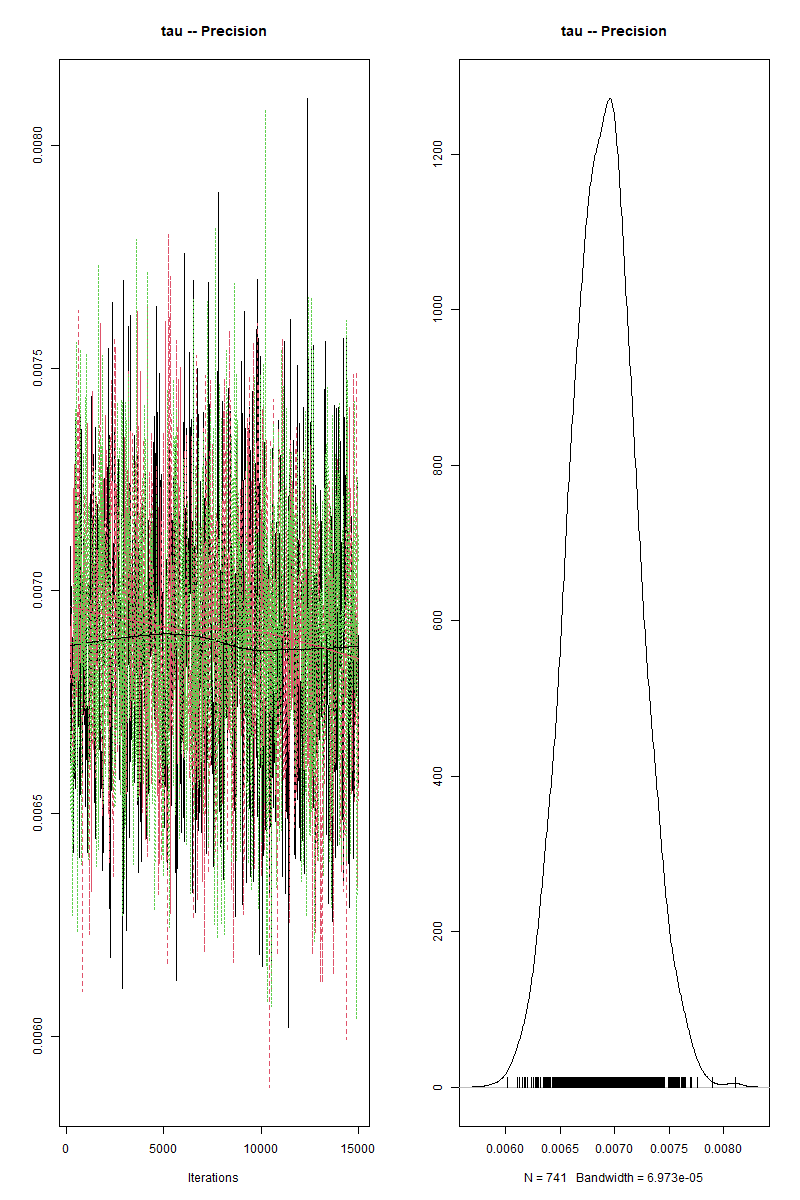
\includegraphics[width=0.7\linewidth]{img/img-trace-tao}
	\caption{Trace and posterior density plots for the parameter $\tau$ (precision of the normal likelihood). The trace plot shows good chain mixing and stationarity across all three chains, with no divergence, drift, or separation after burn-in. Fluctuations are consistently centred around a stable mean, showing convergence. The posterior density plot reveals a narrow and sharply peaked unimodal distribution concentrated between approximately 0.0063 and 0.0078, peaking near 0.0069, showing a tightly constrained estimate of the model’s residual precision. The rug plot below the density curve confirms dense and stable sampling from the posterior. This supports reliable inference for the precision parameter $\tau$.}
	\label{fig:img-trace-tao}
\end{figure}


\begin{figure}[H]
	\centering
	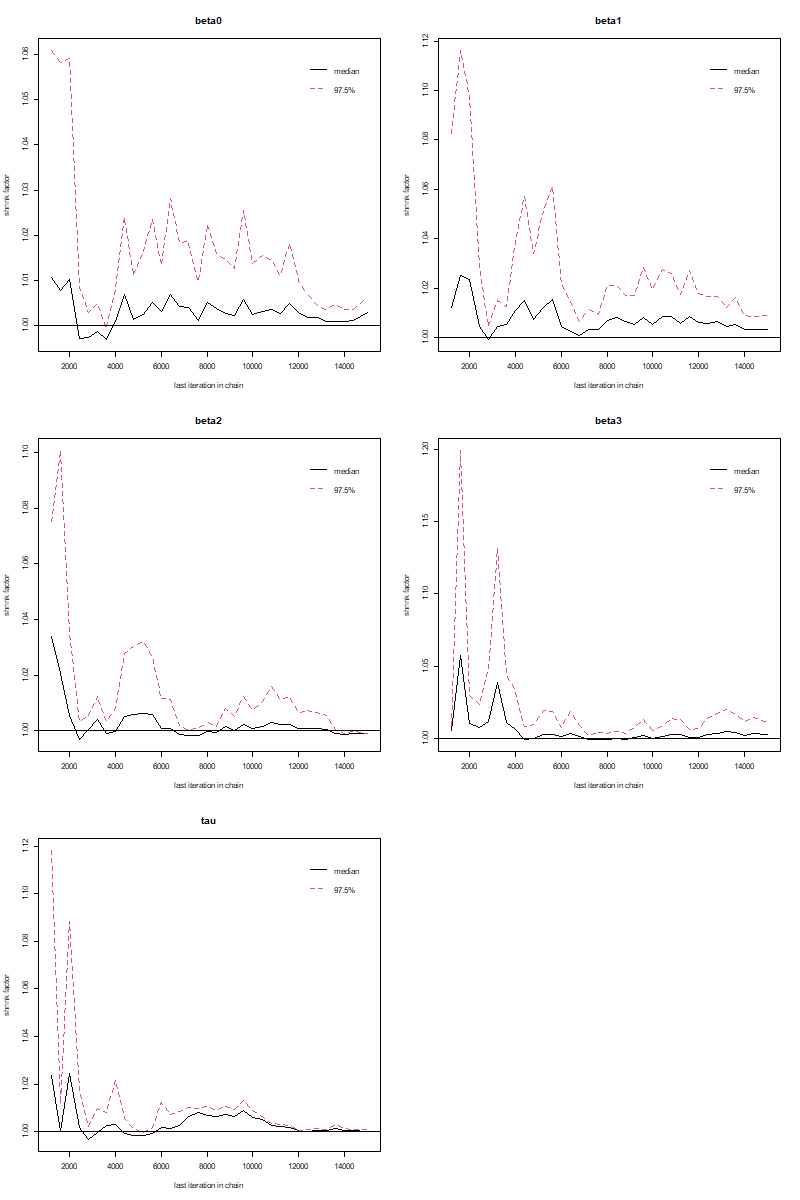
\includegraphics[width=0.7\linewidth]{img/img-gelman-plot-all}
	\caption{Gelman--Rubin diagnostic plots for all monitored parameters: intercept, cement, superplasticizer, age, and precision. The plots show the evolution of the shrink factor across increasing chain lengths. All parameters converge to Potential Scale Reduction Factor values close to 1.00 with their 97.5\% confidence intervals stabilising below 1.05. Convergence for all parameters appears to occur around iteration 6000, after which the shrink factors remain flat and close to unity. This shows that the chains for all parameters have likely converged to the same posterior distribution and that no substantial between-chain variation remains.}
	\label{fig:img-gelman-plot-all}
\end{figure}


\begin{figure}
	\centering
	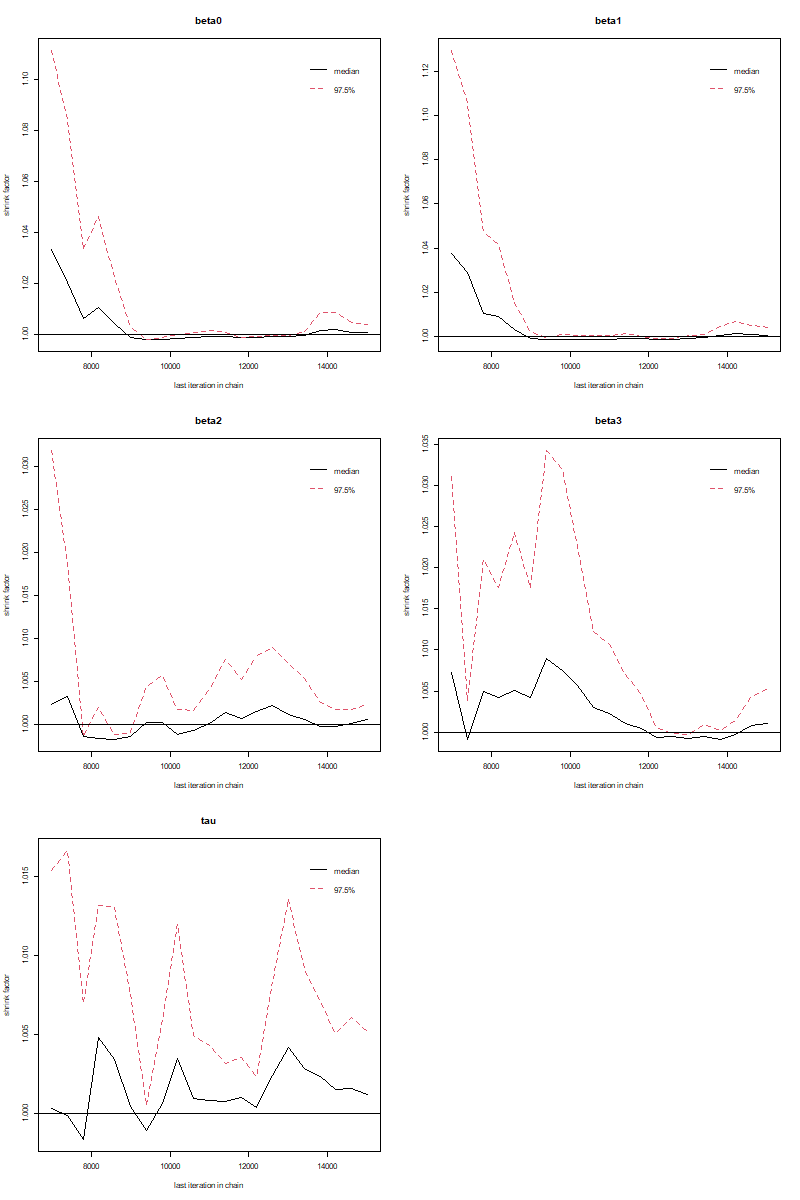
\includegraphics[width=0.7\linewidth]{img/img-gelman-plot-all-bi}
	\caption{Gelman-Rubin diagnostic plots for all monitored parameters following the removal of the first 6000 iterations as burn-in. After burn-in, all parameters show Potential Scale Reduction Factor values stabilising near 1.00, with their 97.5\% confidence intervals remaining below 1.05, indicating convergence. This confirms that discarding the initial 6000 iterations was effective in eliminating non-stationary behaviour, and that the retained samples are representative of the joint posterior distribution.}	\label{fig:img-gelman-plot-all-bi}
\end{figure}


\subsection{A discussion of the posterior distributions obtained from the analysis based on the
plots and summary statistics (which need to be presented in the text). Discuss also
how the posterior distributions of the model parameters can be used to predict new
values of the response variable Y, given only values for the explanatory variables
are available (prediction problem). Include both the interpretation of the parameter
uncertainty and how it propagates into predictions for new observations.}

\subsection{Also present the R script, including comments that explain what each section does in
an appendix. }



\end{document}
